\begin{frame}{La bataille navale}
  \scriptsize
    \begin{columns}
      \column{0.6\textwidth}
        Jouons à la bataille navale avec un(e) partenaire.
        Voici les règles:
        \begin{itemize}
          \item Tu auras 4 bateaux qui prennent les nombres de cases \gloss{squares} suivants:
          \begin{itemize}
            \scriptsize
            \item 2 cases, 3 cases, 4 cases, 5 cases
          \end{itemize}
          \item Mets tes bateaux où que \gloss{wherever} tu veux sur le plateau.
          \item Ton/ta partenaire va deviner une case, où se trouve peut-être un de tes bateaux, en construisant une phrase d'un mot de la colonne, un mot de la ligne \alert{et un nom approprié pour la phrase}.
          \begin{itemize}
            \scriptsize
            \item Par ex., Tu + manquer de quoi $\to$ Tu manques de temps
          \end{itemize}
          \item Il faut utiliser \textcolor{red}{un nom différent} chaque fois, mais il peut être n'importe quel nom.
          \item Si c'est une case où tu as un bateau, marque la case.
          \item Si toutes les cases d'un bateau sont choisies, le bateau est coulé \gloss{sunk}.
          \end{itemize}
      \column{0.4\textwidth}
        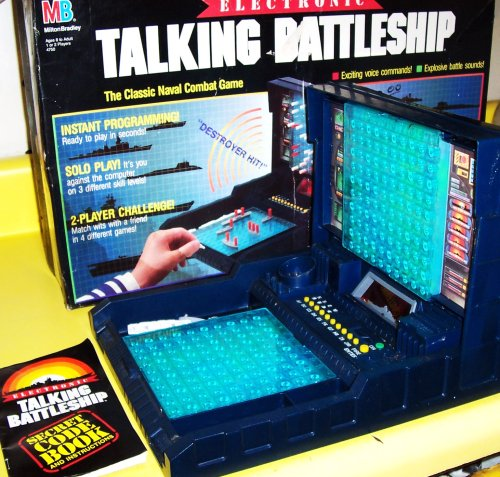
\includegraphics[scale=0.25]{battleship.jpg}
    \end{columns}
\end{frame}